\documentclass[11pt,a4paper]{article}
\usepackage[latin1]{inputenc}
\usepackage{amsmath}
\usepackage{amsfonts}
\usepackage{amssymb}
\usepackage{graphicx}
\usepackage{longtable}
\usepackage{tabularx}
\usepackage{enumitem}
\usepackage{url}
\usepackage[margin=0.8in]{geometry}
\usepackage[toc,page]{appendix}
\usepackage{etoolbox}
\usepackage{morefloats}
\usepackage[hidelinks]{hyperref}
\usepackage{float} % Allows putting an [H] in \begin{figure} to specify the exact location of the figure


\graphicspath{{img/}}

\patchcmd{\thebibliography}{\section*}{\subsection}{}{}

% Table padding
\renewcommand{\arraystretch}{1.5}

\begin{document}

\begin{titlepage}

\begin{center}

\includegraphics[width=0.5\textwidth]{img/University_Logo}\\

\textsc{\LARGE Swansea University }\\[0.5cm]
\textsc{\large MEng Computing }\\[2cm]

{ \huge \bfseries Group Project CS-M04}\\[0.2cm]
\textsc{\large Team Structure, Methodology, Requirements and Specifications}\\[1.5cm]

\begin{minipage}{0.4\textwidth}
\begin{flushleft}

\emph{Authors:}\\
Adam \textsc{Barrell} {\scriptsize \emph{(632975)}} \\
Thomas \textsc{Milner} {\scriptsize \emph{(637755)}} \\
Lewis \textsc{Hancock} {\scriptsize \emph{(xxxxxx)}} \\
Christopher \textsc{Lewis} {\scriptsize \emph{(xxxxxx)}} \\

\end{flushleft}
\end{minipage}
\begin{minipage}{0.4\textwidth}
\begin{flushright}

\emph{Supervisor:}\\
Parisa \textsc{Eslambolchilar}

\end{flushright}
\end{minipage}\\[1.3cm]

{\today}
\end{center}

\end{titlepage}

\tableofcontents

\section{Introduction}
\subsection{Purpose}
\label{sec:purpose}
The purpose of this document is to explain in great detail the requirements and specifications for the White Rock Digital Trails application. This document was originally created to allow for the development team of Digital Trails and any interested parties within the White Rock organisation.

\subsection{Client Background}
\label{sec:client-background}
White Rock Trails is a recent initiative in the Swansea area to create self-guided digital trails in Swansea's former industrial areas of White Rock and Hafod. 

TODO: wait for reply from John.

\subsection{Scope}
\label{sec:scope}
Digital Trails is a self-guided trail application which was initially created by students at Aberystwyth University before being handed to this team. The development team will be modifying the current code-base and implementing new features to improve the usability and functionality of the application.

These modifications include, but are not limited to:
\begin{itemize}
\item Replace OpenStreetMap with Google Maps.
\item Improving the usability of the application.
\item Allow real-time collection of GPS waypoints.
\item Allow real-time collection of geotagged photographs and other media.
\item Expand compatibility to a wide range of android tablets.
\item Enable social-media interactions within the application.
\end{itemize}

The database which stores the trails will also be modified so it can be found remotely on the tablet and modified when a user wants to add or remove trails from their application.

The development team will also be creating a web portal to allow for the creation new trails. Any user with a registered account will be able to create and modify their own walks to share with the rest of the user-base.

\subsection{Term Definitions}
\label{sec:terms}

\subsubsection{OpenStreetMap}
An open-source collaborative project which aims to create a free map of the world~\cite{OSM}.

\subsubsection{Google Maps}
A web mapping service provided by Google. It powers multiple map-based services. Digital Trails will be using the Google Maps API~\cite{googleAPI}.

\subsubsection{Geotagging}
The process of adding metadata corresponding to geographical data to media. Usually this data is the location at which the media was created.

\subsubsection{Metadata}
Data which describes data.

\subsubsection{Git}
A distributed version control system which allows the development team to share files and keep track of changes~\cite{git}.

\subsubsection{GitHub}
TODO: write this.

\subsubsection{Android}
A mobile operating system developed by Google~\cite{android}. 

\subsubsection{IDE}
Integrated Development Environment, a software application which provides facilities to assist with software development.

\subsubsection{HCI}
Human-Computer Interaction is the study of the interaction between people and computers.

\subsubsection{UX}
User Experience is a subset of HCI, looking at a person's behaviour and emotions when using a product.

\subsection{Overview}
The latter sections of this document contains the project requirements, specifications, methodology to be used and any identified risks. To begin, the document looks at the team's structure during the project; this may be seen in section~\ref{sec:team-structure}. In section~\ref{sec:gen-desc}. the Digital Trails project is examined at a high level, providing an overview of the system and any constraints upon it. Section~\ref{sec:requirements} contains the requirements of the project whilst section~\ref{sec:specifications} details the specifications. In section~\ref{sec:methodologies} the project's methodology has been described, first examining possible methodologies before stating which one the team will follow. The project's risks have been identified and analysed in section~\ref{sec:risk-analysis}. A timetable for the project can be seen in section~\ref{sec:project-plan}. Finally, the initial work completed on the project is discussed in section~\ref{sec:initial-work}.



\section{Team Structure}
\label{sec:team-structure}
This section will outline our teams structure, detailing which member will be responsible for each aspect and how they will work together. 

\subsection{Roles and Responsibilities}
This project has two major parts, the Mobile App and the Website. This structure lends its self to division of the team into two development groups. The Mobile group will deal with the development and design of the Android App and the Web group will create the web portal and backend web services. The groups will be organised like so;  
\begin{table}[h]
\begin{center}
\begin{tabular}{|c|c|}
\hline
\textbf{Web Group} & \textbf{Mobile Group} \\
\hline
Thomas Milner & Lewis Hancock \\
Adam Barrell & Chris Lewis \\ \hline
\end{tabular}
\end{center}
\end{table}%

The two groups will not work independently, instead they will be co-operating through out the design and development process to ensure that the mobile app and website meet the same requirements and design choices. 

On top of the team allocations each members of the project has been assigned an individual role:

\begin{table}[h]
\begin{center}
\begin{tabular}{|c|c|}
\hline
\textbf{Role} & \textbf{Member} \\
\hline
Project Overlord & Adam Barrell  \\\hline
HCI \& UX Tzar & Chris Lewis \\ \hline
Android Genie & Lewis Hancock \\\hline
Web Guru & Thomas Milner \\\hline
\end{tabular}
\end{center}
\end{table}%

These roles are designed around each members expertise and skills. The Project Overlord is responsible for the general overview and control of the project; scheduling meetings, organising work days, ensuring deadlines are met and liaising with the client (John at White Rock). The HCI \& UX Tzar is in charge of the design process. Their main role is to ensure good UX design through out the project (See section \ref{sec:terms} for definitions of UX and HCI.). The Android Genie will lead the android team and is responsible for the development of the android application. They should ensure the use of good design practices during the development. Finally the Web Guru is responsible for the web team and is in charge of developing the website. The Guru should again ensure the use of good design practices and that the website correctly interacts with the existing framework of the android app. 

\subsection{Communication Strategy}

Communication is an important part of any project. The team will be using several different mediums to communicate with each other, the client and with 3rd parties. The first important medium is Social Media. 

We will be making extensive use of Social media for group communication. This will mainly take place through the Facebook platform, using the Chat system and a private group. This will allow us to talk as a group at any opportunity and to share documents and news. It can be used by the Project Overlord to publish details of meetings and keep us update with important news from the Client and other important parties. 

The second medium is formal meetings. They will be held by the Project Overlord and will be used for decision making by the group as a whole and as part of out methodology to ensure work is on target. Meetings will be scheduled in advance and will generally be held once a week at the end of the current development cycle. Occasionally the Client will be invited to attend meetings, this will mainly occur when the project reaches critical milestones. 

Emails will be the another important communication strategy, they will mainly be used for communication with the client and other 3rd parties such as lecturers who cannot be reached via social media and are not generally accessible for face to face communication. 

Lastly, as the team generally see each other regularly out side of the project, face-to-face communication will commonly be used for less formal discussion between members. 
%%\subsection{Development Strategy}

\section{General Description}
\label{sec:gen-desc}

\subsection{Product Perspective}
\label{sec:product-perspective}
Digital Trails is both an Android application and a web service allowing for the creation, modification and exploration of self-guided digital trails. The application will be capable of running across a range of Android based tablets and is for the use of the general public.

\subsection{Project Overview}
\label{sec:project-overview}


\subsection{Product Functions}
\label{sec:product-functions}


\subsection{User Characteristics}
\label{sec:user-characteristics}


\subsection{Constraints}
\label{sec:constraints}


\subsection{Assumptions and Dependencies}
\label{sec:assumptions-dependencies}

\section{Requirements}
\label{sec:requirements}
\subsection{Functional}
\label{sec:func-reqs}
\subsubsection{Web Portal}
\label{sec:req-reg-login}

\begin{longtable}{|p{2.5cm}p{13cm}|}
\hline
\textbf{Code} & \textbf{Requirement} \\
\hline
WEBREQ1 & The web portal should allow users to register a new account. \\ \hline
WEBREQ2 & The web portal should allow registered users to log in. \\ \hline
WEBREQ3 & The web portal should allow registered users to log out. \\ \hline
WEBREQ4 & The web portal should allow registered users to modify their account details. \\ \hline
WEBREQ5 & The web portal interface should feature distinctive White Rock branding. \\ \hline
WEBREQ6 & The web portal should allow registered users to add sub-branding to created walks. \\ \hline
WEBREQ7 & The web portal should display a registered user's own walks and contributions when logged in. \\ \hline
WEBREQ8 & The web portal should allow registered users to create, edit and delete their own walks. \\ \hline
WEBREQ9 & The web portal should allow registered users to create, edit and delete their own waypoints. \\ \hline
WEBREQ10 & The web portal should allow registered users to add GPS waypoints to a walk. \\ \hline
WEBREQ11 & The web portal should allow registered users to modify the order each waypoint should be visited. \\ \hline
WEBREQ12 & The web portal should allow registered users to upload, edit and delete waypoint data such as images, text, audio and video. \\ \hline
WEBREQ13 & The web portal should allow registered users to provide English and Welsh translation for text. \\ \hline
WEBREQ14 & The web portal should display download statistics for each of the user's walks. \\ \hline
WEBREQ15 & The web portal should display reviews for each of the user's walks. \\ \hline
WEBREQ16 & The web portal should display an average rating for each of the user's walks. \\ \hline
WEBREQ17 & The web portal should notify registered users of waypoint addition requests. \\ \hline
WEBREQ18 & The web portal should allow registered users to accept or reject requested waypoint additions. \\ \hline
WEBREQ19 & The web portal should allow registered users to report bugs and errors. \\ \hline
WEBREQ20 & The web portal should contain an FAQ and user guide. \\ \hline

\end{longtable}

\subsubsection{Android Application}

\begin{longtable}{|p{2.5cm}p{13cm}|}
\hline
\textbf{Code} & \textbf{Requirement} \\
\hline
APPREQ1 & The application should allow users to register user accounts. \\ \hline
APPREQ2 & The application should allow registered users to log in. \\ \hline
APPREQ3 & The application should allow registered users to log out. \\ \hline
APPREQ4 & The application should allow registered users to modify their account details. \\ \hline
APPREQ5 & The application should allow users to download walks created by registered users. \\ \hline
APPREQ6 & The application should group walks by local area. \\ \hline
APPREQ7 & The application should sort grouped walks by current proximity to the user. \\ \hline
APPREQ8 & The application should allow users to use Google earth and street maps interchangeably while viewing a walk. \\ \hline
APPREQ9 & The application should allow registered users to choose a default map view for a created walk. \\ \hline
APPREQ10 & The application should download data from a remote database. \\ \hline
APPREQ11 & The application should synchronise data whilst the host device is connected to WiFi. \\ \hline
APPREQ12 & The application should give users the option to synchronise data over cellular networks. \\ \hline
APPREQ13 & The application should give users the option to store data on an SD card if available. \\ \hline
APPREQ14 & The application should detect a user's GPS location consistently between devices. \\ \hline
APPREQ15 & The application should display the prefered order to visit waypoints in a walk. \\ \hline
APPREQ16 & The application should display waypoint information even if it has already been visited. \\ \hline
APPREQ17 & The application should allow registered users to create, edit and delete their own walks. \\ \hline
APPREQ18 & The application should allow registered users to tag GPS waypoints in their own walks. \\ \hline
APPREQ19 & The application should track the order GPS waypoints were tagged in a created walk. \\ \hline
APPREQ20 & The application should allow registered users to upload audio, images and video to a waypoint. \\ \hline
APPREQ21 & The application interface should separate audio, images, text and video waypoint data. \\ \hline
APPREQ22 & The application interface should feature distinctive White Rock branding. \\ \hline
APPREQ23 & The application should allow registered users to contribute waypoints to other user's walks by request. \\ \hline
APPREQ24 & The application should allow users to leave reviews on walks. \\ \hline
APPREQ25 & The application should allow users to rate walks they have completed. \\ \hline
APPREQ26 & The application should allow users to report bugs and errors. \\ \hline
APPREQ27 & The application should provide links to the app's Twitter and Facebook channels. \\ \hline
APPREQ28 & The application should provide English and Welsh translations for text. \\ \hline
APPREQ29 & The application should allow users to report inappropriate content to an administrator. \\ \hline

\end{longtable}

\subsection{Non-Functional}
\label{sec:non-func-reqs}

\begin{longtable}{|p{2.5cm}p{13cm}|}
\hline
\textbf{Code} & \textbf{Requirement} \\

\hline
NFREQ1 & The web portal must share the same database as the second development group. \\ \hline
NFREQ2 & The application should be intuitive to users with little technology experience. \\ \hline
NFREQ3 & The application should be usable by colour blind and deaf users. \\ \hline
NFREQ4 & The application code should be maintainable for future developers. \\ \hline
NFREQ5 & The application code should be fully documented. \\ \hline
NFREQ6 & The application should run efficiently on lower end GPS-enabled android tablets. \\ \hline
NFREQ7 & The application should run efficiently on android smartphones. \\ \hline
NFREQ8 & The application should be compatible with typical tablet screen sizes. \\ \hline
NFREQ9 & The application should be compatible with typical smartphone screen sizes. \\ \hline
NFREQ10 & The application should be battery efficient by sampling GPS locations based on the user's mode of transport. \\ \hline
NFREQ11 & The application should be bandwidth efficient. \\ \hline
\end{longtable}

\subsection{Nice To Have}


\begin{longtable}{|p{2.5cm}p{13cm}|}
\hline
\textbf{Code} & \textbf{Requirement} \\

\hline
NTHREQ1 & A Facebook channel to enable feedback and contributions from users. \\ \hline
NTHREQ2 & A Twitter channel to enable feedback and contributions from users. \\ \hline
NTHREQ3 & The application should display the latest tweets from the Twitter channel. \\ \hline
NTHREQ4 & The application should allow users to advertise their current walk on Facebook and Twitter. \\ \hline
\end{longtable}

\section{Specifications}
\label{sec:specifications}

\subsection{Functional}
\label{sec:func-specs}

\subsubsection{Web Portal}

\begin{longtable}{|p{2.5cm}p{13cm}|}
\hline
\textbf{Code} & \textbf{Requirement} \\

\hline
WEBSPEC1 & The web portal will have a `Register' button for users which are not logged in. \\ \hline
WEBSPEC2 & Clicking `Register' will display a view with `Name', `Email Address', `Password', `Password Confirmation' text fields and `Register' and `Cancel' buttons.\\ \hline
WEBSPEC3 & Clicking `Cancel' will return the user to the index page.\\ \hline
WEBSPEC4 & Clicking `Register' will create a user, log them in and email them a confirmation. \\ \hline
WEBSPEC5 & There will be a `Login' link on for users that are not logged in.\\ \hline
WEBSPEC6 & Clicking `Login' will present a pop up with `Username' and `Password' fields and `Login' and `Cancel' buttons. \\ \hline
WEBSPEC7 & Clicking `Login' will create an authenticated session for the user stored in a temporary cookie.\\ \hline
WEBSPEC8 & Clicking `Cancel' will dismiss the popup. \\ \hline
WEBSPEC9 & When users are logged in they will be presented with a `Logout' link\\ \hline
WEBSPEC10 & Clicking `Logout' will delete the session cookie and return them to the index page as guest. \\ \hline
WEBSPEC11 & The web portal will feature an `Edit Account' button. \\ \hline
WEBSPEC12 & Clicking the `Edit Account' will display a view that allows the user to edit their `full name, email and password', a `cancel' button and a `save' button. \\ \hline
WEBSPEC13 & Clicking the `Save' button will validate the full name, email and password text boxes. If successful, a notification will inform the user that changes were made to their details. \\ \hline
WEBSPEC14 & Clicking the `Cancel' button will cancel current changes made to the user`s details. \\ \hline
WEBSPEC15 & All web portal views will feature the company logo and use a house colour scheme. \\ \hline
WEBSPEC16 & The `user account settings' view will feature a company branding tab, allowing the user to attach their company logo to a walk. \\ \hline
WEBSPEC17 & The company branding tab will feature a `Browse' button, allowing the user to browse their computer for a particular image and will feature a `Save' button, allowing the user to upload their image. \\ \hline
WEBSPEC18 & Successfully logging in will take the user to a `Homepage' view featuring their own walks and contributions. \\ \hline
WEBSPEC19 & The web portal will feature a `Walk' button on its side bar. \\ \hline
WEBSPEC20 & Clicking the `Walk' button will navigate the user to a view featuring a list of walks and an `Add walk' button. \\ \hline
WEBSPEC21 & Clicking the `Add walk' button will display a view featuring `Walk name, description' textboxes, `Cancel' and `Create' button. \\ \hline
WEBSPEC22 & The `Walk name' and `Description' text boxes will include a profanity filter, preventing inappropriate words being used. \\ \hline
WEBSPEC23 & Clicking the `Cancel' button will navigate the user back to the `Homepage' view. \\ \hline
WEBSPEC24 & Clicking the `Create' button will create a new walk. \\ \hline
WEBSPEC25 & The walk list view will feature an `Edit' button and `Delete' button adjacent to each walk. \\ \hline
WEBSPEC26 & Clicking the `Edit' button will navigate to a view where the user can edit the `Walk name, description' text boxes. \\ \hline
WEBSPEC27 & Clicking the `Delete' button will display a view, asking the user to confirm they wish to delete the walk. \\ \hline
WEBSPEC28 & When in user-walk list view, clicking on a walk will display a view featuring a list of walk waypoints and an `Add waypoint' button. \\ \hline
WEBSPEC29 & Clicking the `Add waypoint' button will display a view featuring `Waypoint name', `Waypoint description' text boxes, `Location Map', `Add image', `Add video' and `Add audio'. \\ \hline
WEBSPEC30 & Clicking the `Add image' button will display a `Browse', `Add' and `Cancel' button. \\ \hline
WEBSPEC31 & Clicking the `Browse' button will allow the user to browse their computer for a suitable image of the waypoint. \\ \hline
WEBSPEC32 & Clicking the `Save' button will upload the image to the waypoint. \\ \hline
WEBSPEC33 & Clicking the `Cancel' button will navigate the user back to the waypoint view. \\ \hline
WEBSPEC34 & Clicking the `Add video' button will display a `Browse', `Add' and `Cancel' button. \\ \hline
WEBSPEC35 & Clicking the `Browse' button will allow the user to browse their computer for a suitable video of the waypoint. \\ \hline
WEBSPEC36 & Clicking the `Save' button will upload the video to the waypoint. \\ \hline
WEBSPEC37 & Clicking a specific point on the `Location map' of the walk will place a waypoint based on its geological location. \\ \hline
WEBSPEC38 & The longitude and latitude co-ordinates must be accepted in the following formats: `British Grid', `Decimal degrees', `Degrees minutes and seconds' and `Degrees and decimal minutes'. \\ \hline
WEBSPEC39 & The waypoint list view will feature an `Edit' button and a `Delete' button adjacent to each waypoint. \\ \hline
WEBSPEC40 & Clicking the `Edit waypoint' button will navigate to a view where the user can edit the `Waypoint name, description' textboxes, waypoint image, waypoint video, waypoint audio and waypoint geological location. \\ \hline
WEBSPEC41 & Each feature of a waypoint shall include a delete button adjacent to the feature. \\ \hline
WEBSPEC42 & Clicking the `Delete' button of a waypoint feature will display a view asking the user if they wish to delete it. For example, clicking the delete button adjacent to the waypoint video will ask the user if they wish to delete the video. \\ \hline
WEBSPEC43 & Clicking the `Delete waypoint' will display a view, asking the user to confirm they wish to delete the waypoint. \\ \hline
WEBSPEC44 & The waypoints view will feature a `Change order' button. \\ \hline
WEBSPEC45 & Clicking the `Change order' button will display a list view of the waypoints, an `Up' button and a `Down' button. \\ \hline
WEBSPEC46 & When a waypoint is selected, clicking the `Up' button will move the waypoint up the list order, clicking the `Down' button will move the waypoint down the list order. \\ \hline
WEBSPEC47 & The web portal side bar will feature a `Translate' button that will display a view featuring `Welsh' and `English' buttons. \\ \hline
WEBSPEC48 & Clicking the `Welsh' button will translate the text into English. \\ \hline
WEBSPEC49 & Clicking the `English' button will translate the text into Welsh. \\ \hline
WEBSPEC50 & The web portal side bar will feature a `Statistics' button, a `Ratings' button, a `Review' button, a `Requests' and a `Report' button. \\ \hline
WEBSPEC51 & Clicking the `Statistics' button navigates the user to a statistics view, displaying each of the user's walks and their download history. \\ \hline
WEBSPEC52 & Clicking the `Ratings' button navigates the user to a ratings view, displaying each of the user's walks and average ratings. \\ \hline
WEBSPEC53 & Clicking the `Reviews' button navigates the user to a review view, displaying each of the user's walks a list of reviews. \\ \hline
WEBSPEC54 & Clicking on the `Request' button navigates the user to a request view, displaying pending waypoints to be added to one of their walks. \\ \hline
WEBSPEC55 & Clicking on a pending waypoint will display a view featuring an `Accept' or `Reject' button. \\ \hline
WEBSPEC56 & Clicking the `Accept' button will add the waypoint to the walk. \\ \hline
WEBSPEC57 & Clicking the `Reject' button will delete the waypoint request. \\ \hline
WEBSPEC58 & Clicking the `Report' button will display a report view, featuring a report/bug `Name', `Description' textboxes, `Send' button and `Cancel' button. \\ \hline
WEBSPEC59 & Clicking the `Send' button will file a report to the White Rock maintenance team. \\ \hline
WEBSPEC60 & Clicking the `Cancel' button will navigate the user to the homepage. \\ \hline
WEBSPEC61 & Clicking the `FAQ' button will navigate to the FAQ. \\ \hline
WEBSPEC62 & The FAQ page shall contain two panels, one for links to question, on the left, and one for answers, on the right. \\ \hline
WEBSPEC63 & The web portal shall have a `Guide' button which links to the User Guide. \\ \hline
WEBSPEC64 & The User Guide page shall contain two panels, one for the contents page, on the left, and one for the guide, on the right. \\ \hline
WEBSPEC65 & The User Guide page will update the guide when the user clicks a link in the contents panel.  \\ \hline
WEBSPEC66 & The User Guide guide panel will contain a back and next button to change the content in the panel. \\ \hline
\end{longtable}

\subsubsection{Android Application}

\begin{longtable}{|p{2.5cm}p{13cm}|}
\hline
\textbf{Code} & \textbf{Requirement} \\

\hline
APPSPEC1 & The app's login view will feature a `Register' button. \\ \hline
APPSPEC2 & Clicking the `Register' button will display a view featuring full name, email and password text boxes, `Register' and `Cancel' buttons. \\ \hline
APPSPEC3 & Clicking the `Register' button will validate the full name, email and password text boxes. If successful, the account will be created, user logged in and navigate the user to a personal home view. \\ \hline
APPSPEC4 & Clicking the `Cancel' button will cancel the registration process and navigate the user back to the launch view. \\ \hline
APPSPEC5 & The app's launch view will feature a `Login' button. \\ \hline
APPSPEC6 & Clicking the `Login' button will display a login view featuring email and password text boxes, `Sign In' and `Cancel' buttons. \\ \hline
APPSPEC7 & Clicking the `Sign In' button will validate the email and password text boxes, log the user in and navigate to a personal home view if successful. \\ \hline
APPSPEC8 & Clicking the `Cancel' button will cancel the sign in process and navigate the user back to the launch view. \\ \hline
APPSPEC9 & The personal home view and options menu will feature a `Log Out' button. \\ \hline
APPSPEC10 & Clicking the `Log Out' button will log the user out of the app and navigate to the launch view. \\ \hline
APPSPEC11 & The personal home view and options menu will feature an `Account' button. \\ \hline
APPSPEC12 & Clicking the `Account' button will navigate the user to a view featuring full name, email, password text boxes and `Save', `Cancel' buttons. \\ \hline
APPSPEC13 & Clicking the `Save' button will validate the full name, email, password text boxes and save any changes to the user's account if successful. A notification will be displayed to inform the user of success or failure. \\ \hline
APPSPEC14 & Clicking the `Cancel' button will cancel the process of account modification and navigate the user to the personal home view. \\ \hline
APPSPEC15 & The launch view will feature a `Search' button which is enabled only when the app detects a WiFi connection. \\ \hline
APPSPEC16 & Clicking the `Search' button will navigate the user to a view containing a search text box, `Go' button and list of walks. \\ \hline
APPSPEC17 & Clicking the `Go' button will filter the walk list to display only the walk names with a full or partial match to the search text. \\ \hline
APPSPEC18 & Walk list items will display the walk name, author, partial description, user rating, downloads and `Download' button. \\ \hline
APPSPEC19 & Clicking the `Download' button will download the walk to the user's device and replace the button with a `tick' icon. \\ \hline
APPSPEC20 & The app will group walk list items which are close in proximity together in a sublist with a heading name of the common local area. \\ \hline
APPSPEC21 & Walk list items grouped by local area will be displayed in descending order based on closest proximity to the app user. \\ \hline
APPSPEC22 & An options menu will feature `Google Earth' and `Google Street' buttons which will be accessible whilst viewing a walk. \\ \hline
APPSPEC23 & Clicking the `Google Earth' button will change the current walk's map to the Google Earth view. \\ \hline
APPSPEC24 & Clicking the `Google Street' button will change the current walk's map to the Google Street view. \\ \hline
APPSPEC25 & Walk edit and add views will feature a default map drop down box containing the options `Google Earth' and `Google Street'. \\ \hline
APPSPEC26 & App data will be downloaded through a web API interfacing a remote database which will be hosted on a Linux server.  \\ \hline
APPSPEC27 & App data will be synchronised with a remote database when the app is launched and the device is connected to WiFi. \\ \hline
APPSPEC28 & The app will display a loading view whilst synchronising app data. \\ \hline
APPSPEC29 & The app will feature a settings view containing a toggle button to enable data download over the cellular data network. \\ \hline
APPSPEC30 & Clicking the toggle button will change its state to on or off accordingly and the setting will be saved. \\ \hline
APPSPEC31 & The settings view will feature a drop down box containing the storage options `Internal' and `SD Card'. \\ \hline
APPSPEC32 & Selecting an option from the storage drop down box will save the setting and move data to the chosen location if it has changed. \\ \hline
APPSPEC33 & The app will display a loading view whilst moving app data to a different location. \\ \hline
APPSPEC34 & A location strategy will be re-implemented using the Android location services API. \\ \hline
APPSPEC35 & The app's GPS accuracy will be tested on the target Hudl tablet and a low end Android 2.2 mobile device to ensure consistency. \\ \hline
APPSPEC36 & The walk view will place a graphic over each waypoint on the map containing a number to represent it's preferred visit order. \\ \hline
APPSPEC37 & The walk view will highlight the next waypoint to visit using a different graphic colour. \\ \hline
APPSPEC38 & Waypoint information will be displayed to the user even if the waypoint has previously been visited since the walk view was opened. \\ \hline
APPSPEC39 & The app will feature a `Walk Options' button.\\ \hline
APPSPEC40 & Clicking on the `Walk Options' button will display a view with `Create Walk' button and a list of walks owned by the user. \\ \hline
APPSPEC41 & Each walk in the list will have an `Edit' and `Delete' button.\\ \hline
APPSPEC42 & Clicking the `Create Walk? button will display a view with `walk name, description' text boxes and `Add waypoints', `Create' and `Cancel' buttons.\\ \hline
APPSPEC43 & Pressing an `Edit' button on a walk will bring up the `Edit Walks' view where the user can edit the `Walk name' and `Description' text fields. There will be an `Add waypoint', `Edit Waypoints', `Create' and `Cancel' buttons. \\ \hline
APPSPEC44 & Pressing the `Delete' button will display a model asking the user to confirm the deletion. \\ \hline
APPSPEC45 & Pressing an `Add waypoints' button will bring up a map view where the users can zoom in and move around. Waypoints are positioned by pressing on a location for a couple of seconds. \\ \hline
APPSPEC46 & Waypoints are automatically assigned the order in which they were created. \\ \hline
APPSPEC47 & Once a location has been assigned the `Edit Waypoint' view is displayed.\\ \hline
APPSPEC48 & Pressing the `Edit Waypoints' button will display a list of current waypoints. Each waypoint will have a `Edit' and `Delete' button. \\ \hline
APPSPEC49 & Pressing the `Edit' button will display an `Edit Waypoint' view. \\ \hline
APPSPEC50 & Pressing the `Delete' button will display a model asking the user to confirm the deletion of the waypoint. \\ \hline
APPSPEC51 & The `Edit Waypoints' view displays a map thumbnail of the location, `Name' and `Description' text boxes, an `Upload' button to add images, audio and video, and a gallery of uploaded media. \\ \hline
APPSPEC52 & Pressing on an item in the gallery of uploaded media will show a pop-up model with a `Delete' button. Clicking `Delete' will present another model asking the user to confirm the deletion. \\ \hline
APPSPEC53 & Pressing the map thumbnail will allow the user to change the position of the waypoint. It will show a map with a movable point and `Confirm' and `Cancel' buttons. \\ \hline
APPSPEC54 & The application will feature White Rock branding and designs where appropriate to build the brand image. \\ \hline
APPSPEC55 & When a registered user is viewing a walk there will be an `Edit' button \\ \hline
APPSPEC56 & Pressing the `Edit' button will display the `Edit Walks' view. The `walk name' and `description' fields will be greyed out to prevent editing.\\ \hline
APPSPEC57 & Any edits to walks created by people other than owner will require them to be confirmed by the owner before being published. \\ \hline
APPSPEC58 & When a user has visited every waypoint on a walk a model will appear asking the user if they have finished. It will have `Finished' and `Carry on' buttons. \\ \hline
APPSPEC59 & A user can force a walk to finish by pressing a `Finish' button in the options menu. \\ \hline
APPSPEC60 & Pressing `Finish' displays a view with a `Review' text box, `Submit review' button, 5 star rating system and `Report a bug' button. \\ \hline
APPSPEC61 & Submitting a review submits the data in the `Review' text box and displays it on the walks information page.\\ \hline
APPSPEC62 & Filling in the 5 star rating system will automatically send the result to the server.\\ \hline
APPSPEC63 & Pressing `Report a Bug' will launch the email client. \\ \hline
APPSPEC64 & The `to? address will be set as the email address of the owner, the `subject? field will be set in the format ``BUG REPORT - WALK `NAME' ''.\\ \hline
APPSPEC65 & The app will link to the White Rocks Twitter and Facebook page from the main page.\\ \hline
APPSPEC66 & The application provide an option in the settings view to display welsh text where available. \\ \hline
APPSPEC67 & On each waypoint and walk there will be a `Report' button which will flag the content as inappropriate. \\ \hline
APPSPEC68 & And content which has been flagged as inappropriate will appear to administrators, who can modify or delete it. \\ \hline
\end{longtable}


\subsection{Non-Functional}
\label{sec:non-func-specs}

\begin{longtable}{|p{2.5cm}p{13cm}|}
\hline
\textbf{Code} & \textbf{Requirement} \\

\hline
NFSPEC1 & Database schema shall be agreed with the second development group \\ \hline
NFSPEC2 & The final database will be hosted on a central server. \\ \hline
NFSPEC3 & The user interface shall be well labelled. \\ \hline
NFSPEC4 & The user will follow traditional mobile interface design decisions to reduce the learning curve of the application. \\ \hline
NFSPEC5 & Use the interface of default Android applications where possible. e.g. The Holo-light theme \\ \hline
NFSPEC6 & Create an optional step by step tutorial for first time users. \\ \hline
NFSPEC7 & Create button to access the tutorial in the settings screen. \\ \hline
NFSPEC8 & In the settings view there will be an option to enable colour blind mode. \\ \hline
NFSPEC9 & Colour blind mode will modify the user interface to use a colour pallette usable by the majority of colorblind users. \\ \hline
NFSPEC10 & In the settings view there will be an option to enable a speech to text feature. \\ \hline
NFSPEC11 & The speech to texture feature will turn user submitted audio into on-screen text. \\ \hline
NFSPEC12 & The settings view will contain an option to allow the device to vibrate when approaching a destination along the route. \\ \hline
NFSPEC13 & The settings view will contain an option to allow the device to emit an audible beep when approaching a destination along the route. \\ \hline
NFSPEC14 & Coding conventions shall be enforced. \\ \hline
NFSPEC15 & Unit tests shall be ran and results documented during development. \\ \hline
NFSPEC16 & All code shall be commented, according to conventions. \\ \hline
NFSPEC17 & Code documentation shall be generated by Doxygen. \\ \hline
NFSPEC18 & Compile with Android 2.2 as a minimum Operating System. \\ \hline
NFSPEC19 & Use compatibility libraries to allow for compatibility for both low and high end devices. \\ \hline
NFSPEC20 & Create a dynamic user interface using Fragments. \\ \hline
NFSPEC21 & Sample GPS based on mode of transport the user has input. (update when better idea). \\ \hline
\end{longtable}

\subsection{Nice To Have}

\begin{longtable}{|p{2.5cm}p{13cm}|}
\hline
\textbf{Code} & \textbf{Requirement} \\

\hline
NTHSPEC1 & A Facebook page for the digital trails application will be created to promote the app and enable community feedback. \\ \hline
NTHSPEC2 &  A Twitter page for the digital trails application will be created to promote the app and enable community feedback. \\ \hline
NTHSPEC3 & The Twitter API will be used to access tweets from the app's Twitter page. \\ \hline
NTHSPEC4 & The Facebook API will be used to allow sharing to user Facebook accounts. \\ \hline
NTHSPEC5 & Allow users to link their accounts to their Facebook accounts. \\ \hline
\end{longtable}


\section{Cross References}
\label{sec:cross-refs}

\subsection{Functional}

\subsubsection{Web Portal}

\begin{longtable}{|p{2.7cm}|p{10cm}|}
\hline
\textbf{Requirement Code} & \textbf{Specification Code} \\

\hline \hline RALFREQ1 & RALSPEC1, RALSPEC2, RALSPEC3  \\
\hline 
\end{longtable}


\subsubsection{Android Application}

\begin{longtable}{|p{2.7cm}|p{10cm}|}
\hline
\textbf{Requirement Code} & \textbf{Specification Code} \\

\hline \hline AFAFREQ1 & AFASPEC1, AFASPEC2, AFASPEC3, AFASPEC4, AFASPEC5  \\
\hline 
\end{longtable}


\subsection{Non-Functional}

\begin{longtable}{|p{2.7cm}|p{10cm}|}
\hline
\textbf{Requirement Code} & \textbf{Specification Code} \\

\hline \hline NFREQ1 & NFSPEC1\\
\hline 
\end{longtable}

\section{Methodology}
\label{sec:methodologies}

\subsection{Considered Methodologies}

\subsubsection{Spiral}
This section is a modified version of the work found in ``A RESTful Document Archival System''~\cite{restWeb}. The spiral methodology is a risk based system, which works iteratively towards a final working project. The process derives its name from the pattern with which its process follows. There are 4 basic activities which must occur in cycle loop of the spiral\ref{img:spiral}. These are:

\begin{enumerate}
  \item Consider all success-critical win conditions.
  \item Identify and evaluate alternative methods for meeting win conditions.
  \item Identify and resolve risks caused by the methods for meeting win conditions. 
  \item Obtain the approval of stakeholders and their commitment to the next cycle. 
\end{enumerate}

\begin{figure}[h]
\begin{center}
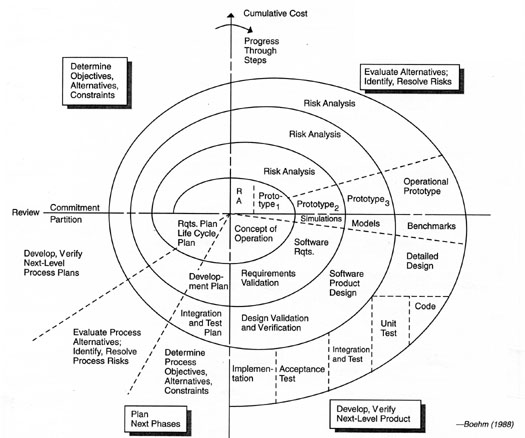
\includegraphics[scale=2.5]{spiral.jpeg}
\label{img:spiral}
\caption{The spiral model \cite{spiral}}
\end{center}
\end{figure}

By identifying risks at each cycle the model allows the developers to decide on the best approach for that cycle and minimise the chance of failure through correct mitigation of those risks. 

This model requires the use of iterative development techniques. This helps force developers to make improvements to previous implementations and requirements, but the exact nature of the iterations are down to interpretation based upon the risks of the project.

Over all spiral is provides a good way of minimising risks in a project but it also has its down sides. It is possible that it it could be executed as simple cycle of waterfall development, this is not the intended use of the the project and is rarely the correct thing to do for the given risks of a project. It could also create an overly complex development strategy which becomes confusing to the development team. This complexity is one of the main arguments against the Spiral model and is addressed by other more agile methods. 

\subsubsection{Prototyping}

\subsubsection{Extreme Programming}
This section has been taken, verbatim, from ``FormulaVis: System Requirements Specification''~\cite{formulaVis}. Extreme Programming is an agile development model aimed at improving the software quality by ensuring a fast and efficient response to changing requirements.

This model advocates frequent releases, similar to sprints in the SCRUM model, which improve productivity and create checkpoints where requirements can be reviewed and adapted. Other elements include pair programming, code reviews and unit testing of all code. Features should not be developed, in this model, until they are needed.

Development cycles begin with a Planning Game, a meeting that occurs at the begin of each cycle. This is divided into two tasks, release planning which determines the requirements to be included in this cycle and when the cycle should end. This phase includes the customer. The second phase is the iteration planning phase, in this phase the requirements are translated into tasks and assigned to programmers. These are then completed before the end of the cycle.

During implementation programmers usually work in pairs and unit tests should be programmed first, then code made to ensure those unit tests pass. This initial code may be inelegant and should be optimised at a later date. If code does not pass the unit tests
then it may not be released. A diagram of the process can be seen in figure~\ref{xp}.

\begin{figure}[H]
\centering
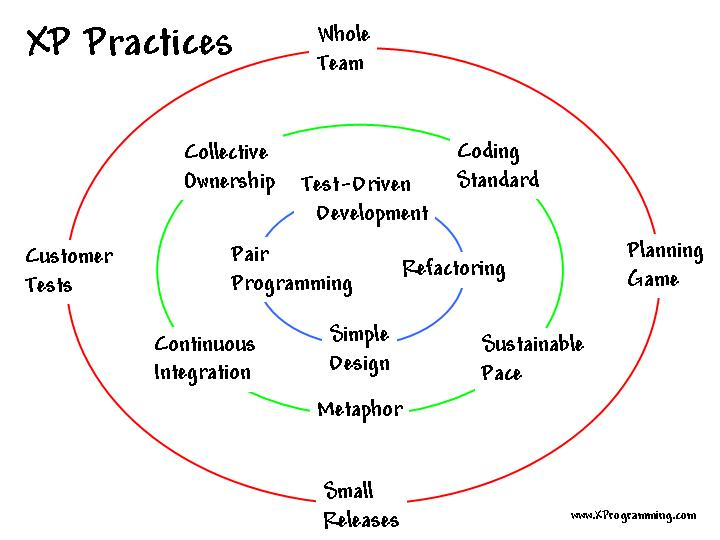
\includegraphics[width = 140mm]{circles.jpg}
\caption{Extreme Programming Model}
\label{fig:xp}
\end{figure}

Critics argue that this practice suffers from unstable requirements and a lack of documentation. The addition of a customer representative as part of the development team can also create feature creep, resulting in a project which runs out of time and
money. The customer representative can also become a point of stress for the team, or a single point of failure for the entire project. Change-control boards are created to prevent this, a sign that there can be conflicts in project objectives. Many more criticisms can be found in Extreme Programming Refactored~\cite{xpRefactored}.


\subsubsection{Crystal Clear}

\subsubsection{SCRUM}

\subsection{Chosen Development Methodology}
TODO: Why we chose scrum

\subsection{Software Testing}
Unit Testing
	regression
	Black Box
Compatibility Testing
Acceptance Testing
User Study

\section{Risk Analysis}
\label{sec:risk-analysis}

\subsection{Risk Matrix}

\subsection{Technical Risks}
\label{sec:tech-risks}

\renewcommand{\arraystretch}{1.2}

\noindent\begin{tabular}{@{}p{3.5cm}p{4cm}p{13cm}@{}}
\textbf{Code:} TECRSK1 & \textbf{Likelihood:} High & \textbf{Impact:} Medium \\ 
\multicolumn{3}{@{}p{17cm}|@{}}{\textbf{Risk:} This is a test risk.} \\ 
\multicolumn{3}{@{}p{17cm}@{}}{\textbf{Mitigation:} This is a test risk. } \\ 
\end{tabular} 

\vspace{0.5 cm}

\noindent\begin{tabular}{@{}p{3.5cm}p{4cm}p{13cm}@{}}
\textbf{Code:} TECRSK1 & \textbf{Likelihood:} High & \textbf{Impact:} Medium \\ 
\multicolumn{3}{@{}p{17cm}|@{}}{\textbf{Risk:} This is a test risk.} \\ 
\multicolumn{3}{@{}p{17cm}@{}}{\textbf{Mitigation:} This is a test risk. } \\ 
\end{tabular} 

\subsection{Personal Risks}
\label{sec:personal-risks}

\noindent\begin{tabular}{@{}p{3.5cm}p{4cm}p{13cm}@{}}
\textbf{Code:} PERRSK1 & \textbf{Likelihood:} 4 & \textbf{Impact:} 7 \\ 
\multicolumn{3}{@{}p{17cm}|@{}}{\textbf{Risk:} A member of the team is absent for a substantial amount of time and is therefore not able to contribute to project work. This will cause the work rate to slow and may impact the delivery dates set out in the project timetable.} \\ 
\multicolumn{3}{@{}p{17cm}@{}}{\textbf{Mitigation:} Extra time will be allocated to complete project tasks so delivery dates are not severely impacted if one team member is absent. } \\ 
\end{tabular} 

\vspace{0.5 cm}

\noindent\begin{tabular}{@{}p{3.5cm}p{4cm}p{13cm}@{}}
\textbf{Code:} TECRSK1 & \textbf{Likelihood:} High & \textbf{Impact:} Medium \\ 
\multicolumn{3}{@{}p{17cm}|@{}}{\textbf{Risk:} This is a test risk.} \\ 
\multicolumn{3}{@{}p{17cm}@{}}{\textbf{Mitigation:} This is a test risk. } \\ 
\end{tabular} 

\section{Project Plan}
\label{sec:project-plan}

\subsection{Milestones}
\label{sec:plan-milestones}

\renewcommand{\arraystretch}{1.5}
\newcommand*{\tableIndent}{\hspace*{0.4cm}}

\begin{figure}[H]
\centering
\begin{tabular}{|l|l|l|}
\hline \textbf{Task} & \textbf{Start Date} & \textbf{End Date} \\ 
\hline \hline \textbf{Milestone 1} & 08 Nov 2013 & 13 Dec 2013 \\ 
\hline\tableIndent General Description & 08 Nov 2013 & 13 Nov 2013 \\ 
\hline\tableIndent Software Requirements & 13 Nov 2013 & 18 Nov 2013 \\ 
\hline\tableIndent Software Specifications & 18 Nov 2013 & 22 Nov 2013 \\ 
\hline\tableIndent Development Methodology & 22 Nov 2013 & 27 Nov 2013 \\ 
\hline\tableIndent Risk Analysis & 27 Nov 2013 & 02 Dec 2013 \\ 
\hline\tableIndent Initial Work  & 02 Dec 2013 & 06 Dec 2013 \\ 
\hline\tableIndent Draft Review  & 06 Dec 2013 & 13 Dec 2013 \\ 
\hline\textbf{Milestone 2} & 14 Feb 2014 & 28 Feb 2014 \\ 
\hline\tableIndent Interim Report & 14 Feb 2014 & 21 Feb 2014 \\ 
\hline\tableIndent Draft Review & 21 Feb 2014 & 28 Feb 2014 \\
\hline\textbf{Milestone 3} & 21 Mar 2014 & 09 May 2014 \\ 
\hline\tableIndent Project Poster & 21 Mar 2014 & 28 Mar 2014 \\ 
\hline\tableIndent User Manual & 28 Mar 2014 & 04 Apr 2014 \\ 
\hline\tableIndent Final Report & 04 Apr 2014 & 02 May 2014 \\
\hline\tableIndent\tableIndent Software Design & 04 Apr 2014 & 11 Apr 2014 \\ 
\hline\tableIndent\tableIndent Software Testing & 11 Apr 2014 & 18 Apr 2014 \\ 
\hline\tableIndent\tableIndent Reflective Account & 18 Apr 2014 & 25 Apr 2014 \\
\hline\tableIndent\tableIndent Draft Review & 25 Apr 2014 & 09 May 2014 \\
\hline 
\end{tabular}

\caption{Milestone time table.\label{fig:milestones-table}}
\end{figure}


\subsection{Software Development}
\label{sec:plan-software-dev}

\renewcommand{\arraystretch}{1.5}

\begin{figure}[H]
\centering
\begin{tabular}{|l|l|l|}
\hline \textbf{Task} & \textbf{Start Date} & \textbf{End Date} \\ 
\hline\hline\textbf{Initial Requirements} & 01 Oct 2013 & 11 Oct 2013 \\
\hline\tableIndent Background Research & 01 Oct 2013 & 04 Oct 2013 \\ 
\hline\tableIndent User Interviews & 04 Oct 2013 & 11 Oct 2013 \\ 
\hline\textbf{Paper Prototypes} & 11 Oct 2013 & 31 Oct 2013 \\
\hline\tableIndent Prototype Development & 11 Oct 2013 & 21 Oct 2013  \\
\hline\tableIndent Wizard of Oz Experiments & 21 Oct 2013 & 23 Oct 2013  \\ 
\hline\tableIndent Revision \& Enhancement & 23 Oct 2013 & 31 Oct 2013 \\  
\hline\textbf{Static HTML Pages} & 31 Oct 2013 & 22 Nov 2013 \\ 
\hline\tableIndent Prototype Development & 31 Oct 2013 & 14 Nov 2013  \\
\hline\tableIndent Cognitive Walkthrough Experiments & 14 Nov 2013 & 17 Nov 2013  \\ 
\hline\tableIndent Revision \& Enhancement & 17 Nov 2013 & 22 Nov 2013  \\ 
\hline\textbf{Service Simulation} & 13 Dec 2013 & 29 Jan 2014 \\
\hline\tableIndent Prototype Development & 13 Dec 2013 & 10 Jan 2014 \\
\hline\tableIndent Prototype Feedback & 10 Jan 2014 & 15 Jan 2014 \\ 
\hline\tableIndent Revision \& Enhancement & 15 Jan 2014 & 22 Jan 2014  \\
\hline\tableIndent Software Testing & 22 Jan 2014 & 29 Jan 2014 \\ 
\hline\textbf{Service Implementation} & 29 Jan 2014 & 14 Mar 2014 \\ 
\hline\tableIndent Prototype Development & 29 Jan 2014 & 19 Feb 2014  \\ 
\hline\tableIndent Prototype Feedback & 19 Feb 2014 & 21 Feb 2014 \\ 
\hline\tableIndent Revision \& Enhancement & 21 Feb 2014 & 28 Feb 2014 \\
\hline\tableIndent Software Testing & 28 Feb 2014 & 14 Mar 2014 \\ 
\hline 
\end{tabular}
\caption{Software development time table.\label{fig:software-dev-table}}
\end{figure}


\section{Initial Work}
\label{sec:initial-work}

\subsection{Minutes of Meetings}
\subsection{User Interface Wire Frames}
\subsection{Future Work}
\label{sec:future-work}

%References as subsection
\newpage
\bibliographystyle{plain}
\bibliography{bibliography}
\end{document}